\chapter{METODOLOGI}

% Ubah konten-konten berikut sesuai dengan isi dari metodologi

\section{Metode yang digunakan}

Berikut ini adalah metode yang digunakan

% Contoh input gambar dengan format *.jpg
\begin{figure} [H] \centering
  % Nama dari file gambar yang diinputkan
  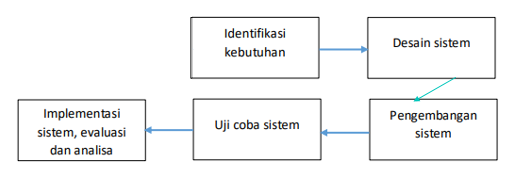
\includegraphics[scale=0.45]{gambar/Screenshot 2023-06-10 193529.png}
  % Keterangan gambar yang diinputkan
  \caption{Metodologi Penelitian}
  % Label referensi dari gambar yang diinputkan
  \label{fig:Metodologi}
\end{figure}

% Contoh penggunaan referensi dari gambar yang diinputkan
Gambar \ref{fig:Metodologi} menjelaskan tentang metodologi penelitian.

\section{Bahan dan peralatan yang digunakan}
Dalam penelitian ini, digunakan bahan dan peralatan yang dibutuhkan.
\subsection {Perangkat keras (hardware)}
Perangkat keras yang digunakan adalah sebagai berikut.
\begin{itemize}
 \item Laptop
 \item Mikrokontroler ESP32
 \item \emph{Webcam}
\end{itemize}

\subsection {Perangkat lunak (software)}
Perangkat lunak yang digunakan adalah sebagai berikut.
\begin{itemize}
 \item Arduino IDE
 \item Visual Studio Code
 \item GitHub
\end{itemize}


\section{Urutan pelaksanaan penelitian}

% Ubah tabel berikut sesuai dengan isi dari rencana kerja
\newcommand{\w}{}
\newcommand{\G}{\cellcolor{gray}}
\begin{table}[H]
  \captionof{table}{Tabel timeline}
  \label{tbl:timeline}
  \begin{tabular}{|p{3.5cm}|c|c|c|c|c|c|c|c|c|c|c|c|c|c|c|c|}

    \hline
    \multirow{2}{*}{Kegiatan} & \multicolumn{16}{|c|}{Minggu}                                                                       \\
    \cline{2-17}              &
    1                         & 2                             & 3  & 4  & 5  & 6  & 7  & 8  & 9  & 10 & 11 & 12 & 13 & 14 & 15 & 16 \\
    \hline

    % Gunakan \G untuk mengisi sel dan \w untuk mengosongkan sel
    Pengambilan data          &
    \G                        & \G                            & \G & \G & \w & \w & \w & \w & \w & \w & \w & \w & \w & \w & \w & \w \\
    \hline

    Pengolahan data           &
    \w                        & \w                            & \w & \w & \G & \G & \G & \G & \w & \w & \w & \w & \w & \w & \w & \w \\
    \hline

    Analisa data              &
    \w                        & \w                            & \w & \w & \w & \w & \w & \w & \G & \G & \G & \G & \w & \w & \w & \w \\
    \hline

    Evaluasi penelitian       &
    \w                        & \w                            & \w & \w & \w & \w & \w & \w & \w & \w & \w & \w & \G & \G & \G & \G \\
    \hline
  \end{tabular}
\end{table}


